\section{1-Wire protokol}
%https://www.maximintegrated.com/en/products/digital/one-wire.html
Sensoren benytter en 1-Wire forbindelse til at kommunikere med mikroprocessoren. 1-Wire er en teknologi hvor en  enkelt serial forbindelse fungerer som dataforbindelse i begge retninger. Dette gøres ved at forbinde sensorens datalinie med mikroprocessoren, og en pull-up modstand forbundet til positiv forsyning, som det ses på figur \ref{one_wire_schematic}. 

\begin{figure}[h!]
  \centering
  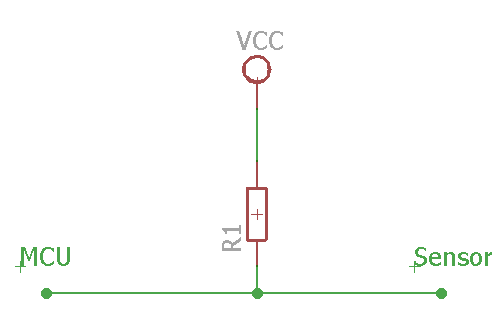
\includegraphics[width=0.4\textwidth]{figures/onewire_eksempel.png}
  \caption{1-Wire data forbindelse mellem sensor og mikroprocessor}
  \label{one_wire_schematic}
\end{figure}

1-Wire fungerer lidt anderledes end en normal data forbindelse. Data bliver læst ud fra tiden hvor der er et 0 V signal, og pull-op modstanden vil trække signalet højt når pinnen er sat til input. Der vil ligge 5 V på dataforbindelsen indtil enten sensor eller mikroprocessor begynder at sende 0 V, hvor den anden enhed så kan registrere hvor længe der ligger 0 V på dataforbindelsen. Tidslængden af 0 V signalet afgør om den enhed der modtager signalet skal opfatte det som et 0 eller 1. Hvis der skal skrives et 0 udsendes der et 0 V signal i 60 $\mu$S og hvis der skal skrives 1 sendes der 0 V i 15 $\mu$S. 

\begin{figure}[h!]
  \centering
  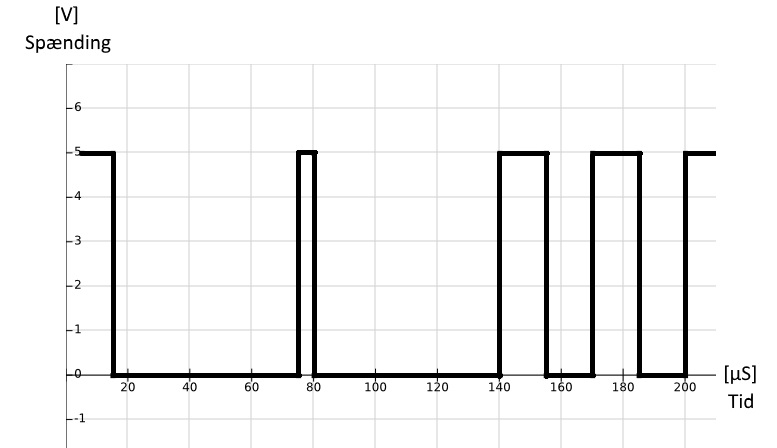
\includegraphics[width=0.7\textwidth]{figures/onewire.png}
  \caption{Teoretisk 1-Wire graf der viser hvad der ligger på dataforbindelsen når der bliver skrevet 0xC.}
  \label{onewire_graph}
\end{figure}
Når der skal læses over 1-Wire sker dette 30 $\mu$S efter en registreret faldet spænding. Det vil sige at da 0 svarer til et delay på 60 $\mu$S vil der måles 0 V her og da 1 svarer til et delay på maksimum 15 $\mu$S vil der læses 5 V eller et højt signal her.
\\
\\
På figur \ref{onewire_graph} ses det hvordan det vil se ud hvis man ønsker at sende hex-tallet 0xC over 1-Wire forbindelsen. Det binære tal for 0xC er 1100 og da 1-Wire skriver fra LSB(Least Significant Bit), skal det ses bagfra. Dette ses på grafen som 2 "store" mellemrum hvor der bliver skrevet 0 V på dataforbindelsen som er efterfuldt af to "korte" som svarer til to 1-taller. \newline Dette er blevet eftermålt med et oscilloskop og kan ses på figur \ref{SCR02}.


\begin{figure}[h!]
  \centering
  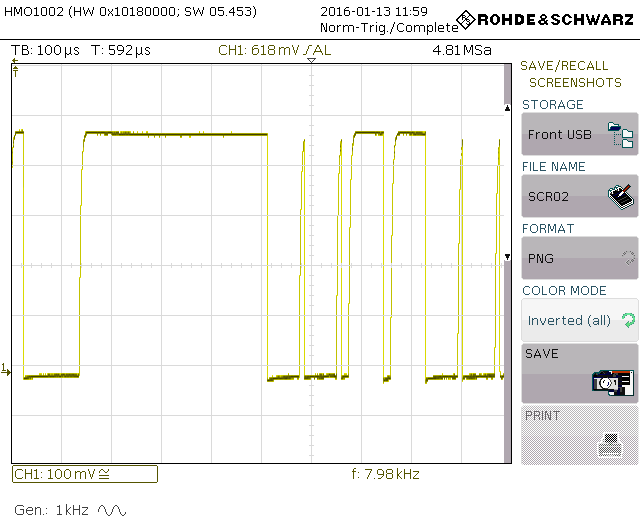
\includegraphics[width=0.7\textwidth]{figures/SCR02.png}
  \caption{Måling af 1-Wire data forbindelse med et oscilloskop.}
  \label{SCR02}
\end{figure}

Figuren viser hvad der måles på dataforbindelsen når mikroprocessoren skriver SKIPROM kommandoen til sensoren.
Fra ca. midten af figuren ses det at SKIPROM funktionen består af 0xCC eller 1100 1100 i binær. Starten af 1100 (læst fra LSB) ses i midten af grafen.